Die in Abbildung \ref{boxplots} dargestellten Boxplots zeigen die Ergebnisse der insgesamt 9 Testreihen aufgeteilt auf die drei Leistungsklassen (LOW, MID, HIGH).


\begin{figure}[h!]
\begin{subfigure}[b]{0.5\textwidth}
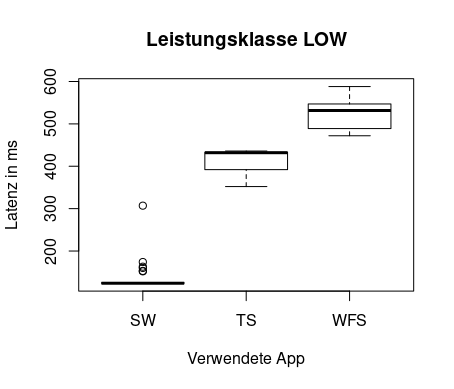
\includegraphics[width=\textwidth]{img/boxplotlow.png}
\end{subfigure}
\begin{subfigure}[b]{0.5\textwidth}
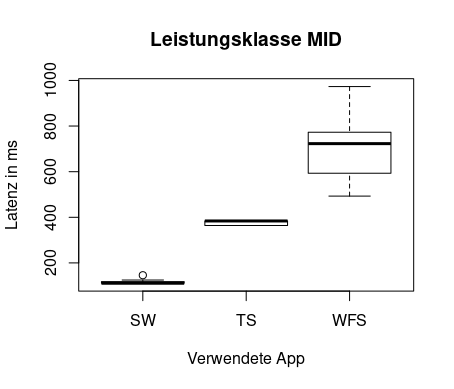
\includegraphics[width=\textwidth]{img/boxplotmid.png}
\end{subfigure}
\begin{subfigure}[b]{0.5\textwidth}
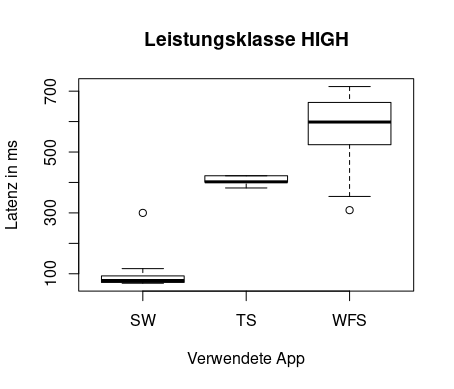
\includegraphics[width=\textwidth]{img/boxplothigh.png}
\end{subfigure}
\caption{Testergebnisse der insgesamt neun Testreihen}
\label{boxplots}
\end{figure}

Nach bloßem Betrachten der Ergebnisse lässt sich die Tendenz verzeichnen, dass bei allen Leistungsklassen SW die geringste Latenz aufweist. Die anschließende statistische Auswertung soll also folgende Hypothesen bestätigen:

\begin{itemize}
\item SW weißt eine geringere Latenz auf als TS.
\item SW weißt eine geringere Latenz auf als WFS.
\end{itemize}

Die Ergebnisse der einzelnen Testreihen wurden dem Shapiro-Wilk Test unterzogen, um auf Normalverteilung zu überprüfen. Nur die Datenreihe der Leistungsklasse LOW und der App WFS verzeichnete dabei einen p-Wert über dem Signifikanzniveau von 0.05 mit einem Wert von 0.06187, wodurch es sich wahrscheinlich um eine Normalverteilung handelt. Bei allen anderen Datenreihen ist anzunehmen, dass diese nicht auf einer Normalverteilung basieren.

In den meisten Datensätzen konnten wir keine Normalverteilung statistisch signifikant feststellen, allerdings sind in jeder Datenreihe 30 Ergebnisse enthalten. Laut \cite{IEEEexample:Georges2007} ist dieser Stichprobenumfang ausreichend, um pro Leistungsklasse einen T-Test zur Überprüfung der Hypothesen durchzuführen. Dabei ist zu beachten, dass der Datensatz von SW jeweils zweimal verwendet wird. Um das Problem des multiplen Testens zu umgehen, wird die Bonferroni-Korrektur angewandt. Dadurch wird das Signifikanzniveau halbiert und somit auf 0.025 gesetzt. Es werden pro Leistungsklasse zwei einseitige T-Tests durchgeführt, welche die Latenzen von SW mit TS und von SW mit WFS vergleichen.

\begin{table}[h]

\begin{tabular}{l|p{2cm}|p{2cm}|p{2cm}}
& LOW & MID & HIGH \\
\hline
SW/TS & t = -35.542; \newline df = 52.287; \newline p-value $< 2.2e-16$ & t = -116.18 \newline df = 51.875; \newline p-value $< 2.2e-16$ & t = -40.896 \newline df = 35.239; \newline p-value $< 2.2e-16$\\
\hline
SW/WFS & t = -44.652; \newline df = 57.64; \newline p-value $< 2.2e-16$ & t = -24.684; \newline df = 29.182; \newline p-value $< 2.2e-16$ & t = -24.806; \newline df = 38.176; \newline p-value $< 2.2e-16$ \\

\end{tabular}
\caption{Ergebnisse der T-Tests}
\end{table}

In allen T-Tests wird das Signifikanzniveau von 0.025 vom p-Wert klar unterschritten. Daraus folgt, dass die vorher aufgestellten Hypothesen akzeptiert werden können. Folgende 95\% Konfidenzintervalle wurden durch die T-Tests berechnet:

\begin{table}[h]

\begin{tabular}{l|p{2cm}|p{2cm}|p{2cm}}
& LOW & MID & HIGH \\
\hline
SW/TS & -Inf -0.2663635 & -Inf -0.2571063 & -Inf -0.3052234 \\
\hline
SW/WFS & -Inf -0.3753667 & -Inf -0.5284751 & -Inf -0.4623933 \\

\end{tabular}
\caption{95\%-Konfidenzintervalle der T-Tests}
\end{table}

Es kann abgelesen werden, dass in 95\% der Fälle die Latenz von SW je nach Leistungsklasse und zu vergleichender App zwischen rund 257ms und 528ms geringer ausfällt.